\documentclass[11 pt, a4paper]{article}
\usepackage[utf8]{inputenc}
\usepackage[italian]{babel} %lingua
\usepackage{textcomp}
\usepackage[a4paper,centering,top=2.5cm,bottom=3.0cm,outer=2.2cm,inner=2.2cm]{geometry}	%%reduce margins
\usepackage{graphicx} %immagini
\usepackage{float} %forza [htb]
\usepackage{listings}
\usepackage{color}
\usepackage{fancyhdr}

\definecolor{mygreen}{rgb}{0,0.6,0}
\definecolor{mygray}{rgb}{0.5,0.5,0.5}
\definecolor{mymauve}{rgb}{0.58,0,0.82}
\definecolor{myblue}{rgb}{0.44,0.62,0.78}


\usepackage[unicode=true]{hyperref} %indice pdf
\hypersetup{breaklinks=true,
pdfauthor={},
pdftitle={},
colorlinks=true,
citecolor=blue,
urlcolor=blue,
linkcolor=black
}

\lstdefinestyle{myRoot}{
backgroundcolor=\color{white},
basicstyle=\footnotesize\ttfamily,        % the size of the fonts that are used for the code
breakatwhitespace=false,         % sets if automatic breaks should only happen at whitespace
breaklines=true,                 % sets automatic line breaking
captionpos=b,                    % sets the caption-position to bottom
commentstyle=\color{mygray},    % comment style
keepspaces=true,                 % keeps spaces in text, useful for keeping indentation of code (possibly needs columns=flexible)
keywordstyle=\color{myblue},       % keyword style
identifierstyle=\color{black},
language=C++,                 % the language of the code
morekeywords={*, TCanvas, Simulator},
numbers=none,                    % where to put the line-numbers; possible values are (none, left, right)
numbersep=5pt,                   % how far the line-numbers are from the code
numberstyle=\tiny\color{mygray}, % the style that is used for the line-numbers
rulecolor=\color{black},         % if not set, the frame-color may be changed on line-breaks within not-black text (e.g. comments (green here))
showspaces=false,                % show spaces everywhere adding particular underscores; it overrides 'showstringspaces'
showstringspaces=false,          % underline spaces within strings only
showtabs=false,                  % show tabs within strings adding particular underscores
stepnumber=2,                    % the step between two line-numbers. If it's 1, each line will be numbered
stringstyle=\color{myblue},     % string literal style
tabsize=2,                     % sets default tabsize to 2 spaces
}

\pagestyle{fancy}
\lhead{}
\cfoot{Francesco Bonacina - Filippo Valle}
\rfoot{\thepage}
\renewcommand{\headrulewidth}{0.3pt}% Remove header rule
\renewcommand{\footrulewidth}{0.3pt}

\author{Francesco Bonacina e Filippo Valle}
\date{\today}
\title{Relazione tans: Protocollo BB84}


\begin{document}
\maketitle

\thispagestyle{empty}
\tableofcontents

\clearpage
\section{Introduzione}
\subsection{BB84, protocollo quantistico di distribuzione delle chiavi per crittografia}
Il BB84 è stato il primo metodo di crittografia quantistica mai inventato ed è utilizzabile come metodo per comunicare in modo privato una chiave segreta tra due utenti per poi utilizzare un protocollo del tipo "cifrario di Vernam" per la crittazione. È stato sviluppato da Charles H. Bennett e Gilles Brassard nel 1984.
\paragraph{Descrizione}
Alice e Bob vogliono riuscire a stabilire una comunicazione sicura per scambiarsi una chiave segreta. La chiave segreta sarà costituita da una stringa di bit $\{0,1\}$, ottenuti misurando qubit negli stati $|0\rangle, |1\rangle, |-\rangle, |+\rangle$, che fisicamente saranno, per esempio, fotoni polarizzati ad angoli rispettivamente di 0°, 90°, -45° e 45°.
Prima dello scambio della chiave segreta Alice e Bob adotteranno il protocollo BB84 per capire se la loro comunicazione è intercettata da qualcuno (Eve). Il protocollo funziona in questo modo:
\begin{itemize}
    \item Alice preparerà un fotone e sceglierà in modo casuale e con uguale probabilità se utilizzare il filtro polarizzatore (\textit{base}) $\{0,1\}$ o quello $\{+,-\}$, inoltre, sempre con probabilità 0.5, codificherà il qbit nello stato 0 o 1 associato a quella base. In questo modo potrà codificare tutti e 4 gli stati possibili. Alice terrà traccia delle basi usate e degli stati preparati.
    \item Il fotone polarizzato verrà trasmesso in un primo canale.
    \item L'eventuale intercettatore Eve riceverà i fotoni di A., cercherà di capire in che stato si trovano misurandoli e poi preparerà nuovi fotoni da trasmettere a B. 
    Eve sa che le basi utilizzate nella codifica sono $\{0,1\}$ e $\{-,+\}$. Quindi ne sceglierà una di queste in modo casuale, farà collassare il qbit intercettato misurandolo e poi trasmetterà a B. un fotone corrispondente alla misura ottenuta.
    \item Il fotone preparato da E. verrà trasmesso a B. in un secondo canale.
    \item Bob a sua volta misurerà i fotoni che riceve utilizzando in modo casuale le basi $\{0,1\}$ e $\{-,+\}$. Anche Bob terrà traccia delle basi usate e degli stati misurati.
    \item Queste operazioni verranno ripetute per tutti gli N fotoni preparati da Alice. Alla fine della trasmissione, Bob comunicherà pubblicamente di aver ricevuto N fotoni e, a quel punto, Alice renderà nota la sequenza degli stati trasmessi e delle basi utilizzate per prepararli. Bob scarterà quindi i fotoni che ha misurato in una base diversa da quella con cui erano stati codificati e vedrà se gli altri qbit si trovano nello stesso stato preparato da Alice. Se alcuni di questi risulteranno alterati, significherà che c'è stata una misura non prevista durante la trasmissione.
\end{itemize}

\begin{figure}[htbp!]
\centering
\includegraphics[width=14cm]{comunicazione_con_Eve2.png}
\end{figure}

\subsection{Trasmissione con rumore}
Nel nostro progetto abbiamo introdotto la possibilità di simulare canali rumorosi. I fotoni trasmessi da Alice a Eve e da Eve a Bob subiscono una variazione di fase di un angolo $\theta$, variabile aleatoria che segue una distribuzione $N(0,\sigma^2)$.
Quindi i qbit, durante la comunicazione, possono risultare alterati oltre che dall'eventuale Eve anche dall'effetto del rumore.

\subsection{Utilizzo di qbit logici}
Per limitare l'effetto del rumore utilizziamo un codice a qbit logici.
Per qbit \textbf{logico} (L) si intende la ripetizione di più qbit fisici (P) identici: nel nostro caso, ad esempio, Alice volendo trasmettere lo stato $|0\rangle$, trasmetterà in realtà lo stato $|000\rangle$. Quindi $|0\rangle_L = |0\rangle_P|0\rangle_P|0\rangle_P$.
Tutti gli attori della comunicazione sono informati dell'utilizzo di qbit logici (anche Eve), quindi sanno che devono aspettarsi "pacchetti" di qbit a tre a tre identici. Chi effettua la misura, tratta indipendentemente i tre qbit nella tripletta. Se i tre valori misurati non sono identici all'interno della singola tripletta, si applicherà una correzione considerando come corretto lo stato con più qbit uguali (es: $|010\rangle$ viene corretto in $|000\rangle$).
Poichè il rumore agisce indipendentemente su ogni qbit, l'utilizzo di qbit logici risulta vantaggioso, infatti la probabilità che vengano alterati almeno due qbit fisici su tre che costituiscono il qbit logico è minore della probabilità che venga alterato il singolo qbit nella comunicazione semplice.

\section{Simulazione}
\subsection{Compilazione ed esecuzione}
Di seguito le istruzioni per eseguire il codice. È possibile compilarlo con \textit{root} o tramite \textit{cmake}.
\subsubsection{Root}
\begin{lstlisting}[language=bash, style=myRoot]
$: root -l compile.C
root [0] 
Processing compile.C...
root [1] .x bb84_simulation.cxx+
\end{lstlisting}

\subsubsection{CMake}
\begin{lstlisting}[language=bash]
$: mkdir build && cd build
$: cmake ..
$: make bb84
$: ./bb84
\end{lstlisting}

\subsection{Struttura del codice}
Il codice è composto da diverse classi, in particolare:
\paragraph{Qbit}
Rappresenta il nucleo della comunicazione, ha come datamember una base che può essere \textit{ZeroOne} o \textit{PlusMinus} e una polarizzazione che può essere \textit{up} o \textit{down}.
Qbit ha al suo interno i metodi per simulare la  preparazione, la misura e l'aggiunta di rumore secondo una funzione data.
I metodi sono automaticamente implementati nel caso di qbit fisici e logici, è sufficiente settare la variabile \textit{fIsLogic}.

\paragraph{Channel}
Serve ad aggiungere, su richiesta, il rumore ai qbit secondo una funzione data.
Possono essere aggiunti un numero variabile di canali.

\paragraph{Phone}
Serve a confrontare i qbit all'inizio e alla fine della comunicazione.

Ha un datamember \textit{fQbitA} in cui vengono salvati i parametri del qbit inviato.

Nucleo della classe è il metodo \textit{MakeCallClassicalChannel} in cui vengono salvati i dati utili nelle successive analisi.

In Phone e in diverse parti del codice si farà riferimento a
\begin{itemize}
\item \textbf{Nsent} è il numero di qbit inviati per \textbf{simulazione}
\item \textbf{SamebasisAltered} è il numero di qbit \textbf{mutati} durante la trasmissione
\item \textbf{SameBasisUntouched} è il numero di qbit che NON sono variati durante la trasmissione
\item \textbf{SamebasisAltered + SameBasisUntouched} è il numero di qbit in cui Alice e Bob hanno utilizzato la stessa base
\end{itemize}

\paragraph{Buddy}
Implementa staticamente funzioni per preparare, intercettare e ricevere un qbit

\paragraph{ConfigSimulator}
Ha come datamember i diversi parametri con cui si può configurare una simulazione.

\paragraph{Simulator}
Simulator si occupa di eseguire una simulazione dati i parametri in un ConfigSimulator e genera i plot che verranno salvati su file.

Vengono simulate comunicazioni di lunghezza variabile e per ogni data lunghezza vengono eseguiti più esperimenti in modo da accumulare statistica.

\paragraph{Analyzer}
Analyzer riceve in input un array di ConfigSimulator con diverse combinazioni dei parametri da testare. Per ognuna di queste costruisce un Simulator con cui eseguire le analisi e poi raggruppa i risultati.

\subsection{Plot e risultati}
Simulator viene creato, vengono eseguite le simulazioni, vengono generati i plot e infine vengono mostrati.
\begin{lstlisting}[language=bash, style=myRoot]
root [0] 
Processing compile.C...
root [1] sim = Simulator::Instance()
root [2] sim->RunSimulation()->GeneratePlots()
root [3] cx = new TCanvas()
root [4] sim->ShowResults(cx)
\end{lstlisting}

Si noti che invocando solo \textit{sim->ShowResults(cx)} è possibile, a simulazione già avvenuta, mostrare solamente i risultati.

\clearpage
\section{Risultati}
\subsection{Esempio di esecuzione di Simulator}

\begin{figure}[htb!]
\centering
\includegraphics[width=0.95\linewidth]{simulator.pdf}
\caption{Esempio di esecuzione simulator}
\label{fig:simulator}
\end{figure}

In figura~\ref{fig:simulator} un esempio di esecuzione di Simulator, da sinistra verso destra si trova:
\begin{itemize}
\item Probabilità che la comunicazione venga alterata in funzione del numero di qbit inviati
\item Numero di qbit alterati in funzione del numero di qbit inviati, in basso la distribuzione per una comunicazione a 50qbit
\item numero di qbit effettivamente utilizzati, in funzione del numero di qbit inviati, in basso la distribuzione a 50 qbit
\end{itemize}

Si nota che in assenza di rumore, con un numero sufficiente di qbit inviati, circa il $50\%$ sono utili alla comunicazione e circa il $25\%$ sono alterati in presenza di Eve.

\clearpage
\subsection{Frazione di qbit alterati in funzione della lunghezza di comunicazione}
Utilizzando la classe \textit{Analyzer} è possibile fare diverse simulazioni cambiano i vari parametri.

In figura~\ref{fig:grafici_LvsP_e_ProbabilityVsN} viene graficato per 4 configurazioni diverse l'andamento della frazione del numero di qbit alterati in funzione del numero di qbit inviati. Il risultato è riportato, per comodità, anche in scala logaritmica.
\begin{figure}[htb!]
\centering
\includegraphics[width=0.9\linewidth]{grafici_LvsP_e_ProbabilityVsN.png}
\caption{Simulazioni con e senza Eve al variare del rumore}
\label{fig:grafici_LvsP_e_ProbabilityVsN}
\end{figure}

\clearpage
\subsection{Trasmissione con qbit fisici e logici in presenza di rumore, senza Eve}

In figura ~\ref{fig:alteredvsnoise} Si mostrano i risultati ottenuti simulando fino a 50 qbit, con 1000 esperimenti senza Eve.
Il rumore è gaussiano con una $\sigma$ che varia tra zero e $2,4$ radianti.

\begin{figure}[htb!]
\centering
\includegraphics[width=0.9\linewidth]{alterednoise.pdf}
\caption{Simulazioni senza Eve al variare del rumore}
\label{fig:alteredvsnoise}
\end{figure}

Si nota che nel caso di qbit logici la frazione di comunicazioni alterate è minore rispetto al caso di qbit fisici.
Senza rumore ($\sigma=0$) l'utilizzo di qbit logici è inutile, in quanto già con qbit fisici il numero di comunicazioni alterate è nullo.
Asintoticamente invece gli andamenti tendono a $\frac{1}{2}$, ovvero vengono alterati tutti i qbit utili alla comunicazione.

\clearpage
\subsection{Trasmissione con qbit logici, con Eve, variando il rumore}
In figura ~\ref{fig:alteredvsnoiseeve} Si mostrano i risultati ottenuti simulando 50 qbit, con 1000 esperimenti senza Eve.
Il rumore è gaussiano con una $\sigma$ che varia tra zero e $2,4$ radianti.

\begin{figure}[htb!]
\centering
\includegraphics[width=0.9\linewidth]{alterednoiseeve.pdf}
\caption{Simulazioni con Eve al variare del rumore}
\label{fig:alteredvsnoiseeve}
\end{figure}

Si nota che nel caso di qbit logici la frazione di comunicazioni alterate è minore rispetto al caso di qbit fisici.
Come nel caso senza Eve, a $\sigma=0$ l'utilizzo di qbit logici è inutile e asintoticamente gli andamenti tendono a $\frac{1}{2}$.

Rispetto al caso precedente, senza Eve, le curve vengono traslate di $\frac{1}{4}$ verso l'alto, infatti l'eventuale intercettore altera in media il $25\%$ delle comunicazioni.

\newpage
\subsection{Trasmissione con qbit logici, con e senza Eve, al variare del rumore}
In figura~\ref{fig:locical_eve_noeve} vengono confrontati gli andamenti della frazione di qbit alterati in presenza o meno di intercettore. Si nota che l'intercettore altera il $25\%$ delle comunicazioni anche senza rumore.

Inoltre per rumori gaussiani con $\sigma>1.5$, anche senza intercettori la comunicazione è compromessa.

\begin{figure}[htb!]
\centering
\includegraphics[width=0.9\linewidth]{logical_eve_noeve.pdf}
\caption{Simulazioni con e senza Eve al variare del rumore}
\label{fig:locical_eve_noeve}
\end{figure}


\subsection{Deviazione standard in funzione del rumore}
Si studia infine l'andamento della larghezza della distribuzione della frazione di qbit alterati al variare del rumore.

\begin{figure}
\centering
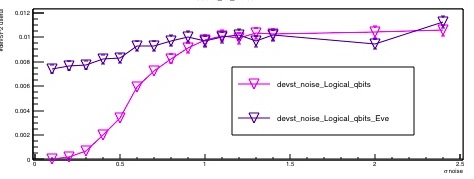
\includegraphics[width=0.9\linewidth]{devstVsNoise.jpeg}
\caption{Anadamento della deviazione standard in funzione del rumore}
\label{fig:devstVsNoise}
\end{figure}

In figura~\ref{fig:devstVsNoise} l'andamento della varianza $\sigma^2$ della curva \textit{Naltered} (la seconda in basso in figura~\ref{fig:simulator}) per diversi rumori.

\end{document}